% vim: ts=4 sts=4 sw=4 et tw=75
% written by dawsunny@github.com originally
\chapter{Algorithms and Data Structures}
\label{chap:alds}
\begin{quote}
    In the end, only familiarity with the tools and techniques of the field
    will provide right solution for a particular problem, and only a
    certain amount of experience will provide consistently professional
    result.
\end{quote}
\begin{quotesrc}
    Raymond Fielding.\bookname{The Technique of Special Effects
    Cinematography}
\end{quotesrc}
The study of algorithms and data structures is one of the foundations of
computer science, a rich field elegant (一流的) techniques and
sophisticated (复杂的) mathematical analyses. And it's more than just fun
and games for the theoretically inclined (倾向于...的): a good algorithm or
data structure might make it possible to solve a problem in seconds that
could otherwise take years.

In specialized areas like graphics, databases, parsing, numerical analysis,
and simulation, the ability to solve problems depends critically on
state-of-the-art (最先进的) algorithms and data structures. If you are
developing your programs in a field that's new to you, you must find out
what is already known, lest (免得) you waste your time doing poorly what
others have already done well.

Every program depends on algorithms and data structures, but few programs
depend on the invention of brand new ones. Even within an intricate
(错综复杂的) program like a compiler or a web browser, most of the data
structures are arrays, lists, trees and hash tables. When a program needs
something more elaborate(详细), it will likely be based on these simpler
ones. Accordingly, for most programmers, the task is to know what
appropriate algorithms and data structures are available and to understand
how to choose among alternatives.

Here is the story in a nutshell. There are only a handful of basic
algorithms that show up in almost every program -- primarily searching and
sorting -- and even those are often included in libraries. Similarly,
almost every data structure is derived (起源) from a few fundamental ones.
Thus the material covered in this chapter will be familiar to almost all
programmers. We have written working versions to make the discussion
concrete, and you can lift (抄) code verbatim (逐字的) if necessary, but do
so only after you have investigated what the programming language and its
libraries have to offer.

\section{Searching}
\label{sec:searching}

Nothing beats an array for storing static tabular (表格式的) data.
Compile-time initialization makes it cheap and easy to construct such
arrays. (In Java, the initialization occurs at run-time, but this is an
unimportant implementation detail unless the arrays are large.) In a
program to detect words that are used rather too much in bad prose (散文),
we can write
\begin{wellcode}
    char *flab[] = {
        "actually",
        "just",
        "quite",
        "really",
        NULL
    };
\end{wellcode}
The search routines needs to know how many elements are in the array. One
way to tell it is to pass length as an argument; another, used here, is to
place a \verb'NULL' marker at the end of the array:
\begin{wellcode}
    /* lookup: sequential search for word in array */
    int lookup(char *word, char *array[])
    {
        int i;
        for (i = 0; array[i] != NULL; i++)
           if (strcmp(word, array[i]) == 0)
                return i;
        return -1;
    }
\end{wellcode}
In C and C++, a parameter that is an array of strings can be declared as
\verb"char *array[]" or \verb"char **array". Although these forms are
equivalent, the first makes it clearer how the parameter will be used.

This search algorithm is called \term{sequential search} because
it looks at each element in turn to see if it's the desired one. When the
amount of data is small, sequential search is fast enough. There are
standard library routines to do sequential search for specific data types;
for example, functions like \texttt{strchr} and \texttt{strstr} search for
the first instance of a given character or substring in a C or C++ string.
The Java \verb'String' class has an \verb'indexOf' method, and the generic
C++ \verb'find' algorithms apply to most data types. If such a function
exists for the data type you've got, use it.

Sequential search is easy but the amount of work is directly proportional
(成比例的) to the amount of data to be searched; doubling the number of
elements will double the time to search if the desired item is not present.
This is a linear relationship -- run-time is a linear function of data size
-- so this method is also known as \term{linear search}.

Here's an excerpt (引用) from an array of more realistic size from a
program that parses HTML, which defines textual names for well over a
hundred individual characters:
\begin{wellcode}
    typedef struct Nameval Nameval;
    struct Nameval{
        char *name;
        int value;
    };
    /* HTML characters, e.g. AElig is ligature of A and E. */
    /* Values are Unicode/ISO10646 encoding. */
    Nameval htmlchars[] = {
        "AElig",    0x00c6,
        "Aacute",   0x00c1,
        "Acirc",    0x00c2,
        /* ... */
        "zeta",     0x03b6,
    };
\end{wellcode}

For a larger array like this, it's more efficient to use \textit{binary
search}. The binary search algorithm is an orderly version of the way we
look up words in a dictionary. Check the middle element. If that value is
bigger than what we are looking for, look in the first half; otherwise,
look in the second half. Repeat until the desired item is found or
determined not to be present.

For binary search, the table must be sorted, as it is here (that's good
style anyway; people find things faster in sorted tables too), and we must
know how long the table is. The \verb'NELEMS' macro from Chapter
\ref{chap:style} can help:
\begin{wellcode}
    printf("The HTML table has %d words\n", NELEMS(htmlchars));
\end{wellcode}

A binary search function for this table might look like this:
\begin{wellcode}
    /* lookup: binary search for name in tab; return index */
    int lookup(char *name, NameVal tab[], int ntab)
    {
        int low, high, mid, cmp;
        low = 0;
        high = ntab - 1;
        while (low <= high){
            mid = (low + high)/2;
            cmp = strcmp(name, tab[mid].name);
            if (cmp < 0){
                high = mid - 1;
            }
            else if (cmp > 0){
                low = mid + 1;
            }
            else{   /* found match */
                return mid;
            }
        }
        return -1;  /* no match */
    }
\end{wellcode}
Putting all this together, to search \verb'htmlchars' we write
\begin{wellcode}
    half = lookup("frac12", htmlchars, NELEMS(htmlchars));
\end{wellcode}
to find the array index of the character $1/2$.

Binary search eliminates half the data at each step. The number of steps is
therefore proportional (成比例的) to the number of times we can divide $n$
by 2 before we're left with a single element. Ignoring roundoff, this is
$\log_2 n$. If we have 1000 items to search, linear search takes up to 1000
steps, while binary search takes about 10; if we have a million items,
linear takes a million steps and binary takes 20. The more items, the
greater the advantage of binary search. Beyond some size of input (which
varies with the implementation), binary search is faster than linear
search.

\section{Sorting}
\label{sec:sorting}

Binary search works only if the elements are sorted. If repeated searches
are going to be made in some data set, it will be profitable to sort once
and then use binary search. If the data set is known in advance, it can be
sorted when the program is written and built using compile-time
initialization. If not, it must be sorted when the program is run.

One of the best all-round sorting algorithms is quicksort, which was
invented in 1960 by C. A. R. Hoare. Quicksort is a fine example of how to
avoid extra computing. It works by partitioning an array into little and
big elements:\\

\indent \indent pick one element of the array (the "pivot").  \\
\indent \indent partition the other elements into two groups: \\
\indent \indent \indent "little ones" that are less than the pivot value,
and   \\
\indent \indent \indent "big ones" that are greater than or equal to the
pivot value.    \\
\indent \indent recursively sort each group.\\

When this process is finished, the array is in order. Quicksort is fast
because once an element is known to be less than the pivot (中枢) value, we
don't have to compare it to any of the big ones; similarly, big ones are
not compared to little ones. This makes it much faster than the simple
sorting methods such as insertion sort and bubble sort that compare each
element directly to all the others.

Quicksort is practical and efficient; it has been extensively studied and
myriad (无数的) variations exist. The version that we present here is
just about the simplest implementation but it is certainly not the
quickest.

This \verb'quicksort' function sorts an array of integers:
\begin{wellcode}
    /* quicksort: sort v[0]..v[n-1] into increasing order */
    void quicksort(int v[], int n)
    {
        int i, last;
        if(n <= 1) /* nothing to do */
            return;
        swap(v, 0, rand() % n); /* move pivot elem to v[0] */
        last = 0;
        for(i = 1; i < n; i++)  /*partition */
            if(v[i] < v[0])
                swap(v, ++last, i);
        swap(v, 0, last);   /* restore pivot */
        quicksort(v, last); /* recursively sort */
        quicksort(v + last + 1, n - last - 1); /* each part */
    }
\end{wellcode}
The \verb'swap' operation, which interchanges two elements, appears three
times in \verb'quicksort', so it is best made into a separate function:
\begin{wellcode}
    /* swap: interchange v[i] and v[j] */
    void swap(int v[], int i, int j)
    {
        int temp;
        temp = v[i];
        v[i] = v[j];
        v[j] = temp;
    }
\end{wellcode}

Partitioning selects a random element as the pivot, swaps it temporarily to
the front, then sweeps through the remaining elements, exchanging those
smaller than the pivot ("little ones") towards the beginning (at location
\verb'last') and big ones towards the end (at location \verb'i'), At the
beginning of the process, just after the pivot has been swapped to the
front, \verb'last=0' and elements \verb'i=1' through \verb'n-1' are
unexamined: \\
\begin{center}
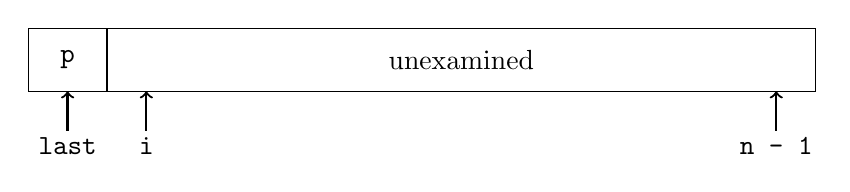
\begin{tikzpicture}
    \draw (0, 0) -- (10, 0);
    \draw (0, 0.8) -- (10, 0.8);
    \draw (0, 0) -- (0, 0.8);
    \draw (1, 0) -- (1, 0.8);
    \draw (10, 0) -- (10, 0.8);
    \node at(0.5, 0.4) {\verb'p'};
    \node at(5.5, 0.4) {unexamined};
    \draw[thick, ->] (0.5, -0.5) -- (0.5, 0);
    \draw[thick, ->] (1.5, -0.5) -- (1.5, 0);
    \draw[thick, ->] (9.5, -0.5) -- (9.5, 0);
    \node at(0.5, -0.7) {\texttt{last}};
    \node at(1.5, -0.7) {\texttt{i}};
    \node at(9.5, -0.7) {\texttt{n - 1}};
\end{tikzpicture}
\end{center}

At the top of the \verb'for' loop, elements \verb'1' through \verb'last'
are strictly less than the pivot (中枢), elements \verb'last+1' through
\verb'i-1' are greater than or equal to the pivot, and elements \verb'i'
through \verb'n-1' have not been examined yet. Until \verb'v[i] >= v[0]',
the algorithm may swap \verb'v[i]' with itself; this wastes some time but
not enough to worry about. \\
\begin{center}
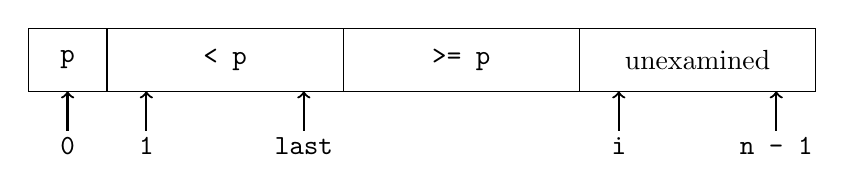
\begin{tikzpicture}
    \draw (0, 0) -- (10, 0);
    \draw (0, 0.8) -- (10, 0.8);
    \draw (0, 0) -- (0, 0.8);
    \draw (1, 0) -- (1, 0.8);
    \draw (4, 0) -- (4, 0.8);
    \draw (7, 0) -- (7, 0.8);
    \draw (10, 0) -- (10, 0.8);
    \node at(0.5, 0.4) {\verb'p'};
    \node at(2.5, 0.4) {\verb'< p'};
    \node at(5.5, 0.4) {\verb'>= p'};
    \node at(8.5, 0.4) {unexamined};
    \draw[thick, ->] (0.5, -0.5) -- (0.5, 0);
    \draw[thick, ->] (1.5, -0.5) -- (1.5, 0);
    \draw[thick, ->] (3.5, -0.5) -- (3.5, 0);
    \draw[thick, ->] (7.5, -0.5) -- (7.5, 0);
    \draw[thick, ->] (9.5, -0.5) -- (9.5, 0);
    \node at(0.5, -0.7) {\texttt{0}};
    \node at(1.5, -0.7) {\texttt{1}};
    \node at(3.5, -0.7) {\texttt{last}};
    \node at(7.5, -0.7) {\texttt{i}};
    \node at(9.5, -0.7) {\texttt{n - 1}};
\end{tikzpicture}
\end{center}

After all elements have been partitioned, element \verb'0' is swapped with
the \verb'last' element to put the pivot element in its final position;
this maintains the correct ordering. Now the array looks like this: \\
\begin{center}
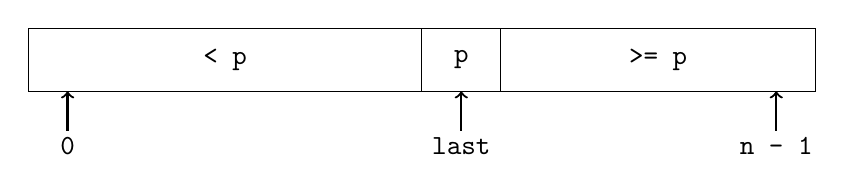
\begin{tikzpicture}
    \draw (0, 0) -- (10, 0);
    \draw (0, 0.8) -- (10, 0.8);
    \draw (0, 0) -- (0, 0.8);
    \draw (5, 0) -- (5, 0.8);
    \draw (6, 0) -- (6, 0.8);
    \draw (10, 0) -- (10, 0.8);
    \node at(2.5, 0.4) {\verb'< p'};
    \node at(5.5, 0.4) {\verb'p'};
    \node at(8, 0.4) {\verb'>= p'};
    \draw[thick, ->] (0.5, -0.5) -- (0.5, 0);
    \draw[thick, ->] (5.5, -0.5) -- (5.5, 0);
    \draw[thick, ->] (9.5, -0.5) -- (9.5, 0);
    \node at(0.5, -0.7) {\texttt{0}};
    \node at(5.5, -0.7) {\texttt{last}};
    \node at(9.5, -0.7) {\texttt{n - 1}};
\end{tikzpicture}
\end{center}

The same process is applied to the left and right sub-arrays; when this has
finished, the whole array has been sorted.

How fast is quicksort? In the best possible case,
\begin{itemize}
\item the first pass partitions $n$ elements into two groups of about $n/2$
    each.
\item the second level partitions two groups, each of about $n/2$ elements,
    into four groups each of about $n/4$.
\item the next level partitions four groups of about $n/4$ into eight of
    about $n/8$.
\item and so on.
\end{itemize}

This goes on for about $\log_2 n$ levels, so the total amount of work in
the best case is proportional to $n + 2\times n/2 + 4\times n/4 + 8\times
n/8 ... $ ($\log_2 n$ terms), which is $n\log_2 n$. On the average, it does
only a little more work. It is customary (习惯的) to use base 2 logarithms;
thus we say that quicksort takes time proportional to $n\log n$.

This implementation of quicksort is the clearest for exposition, but it has
a weakness. If each choice of pivot splits the element values into two
nearly equal groups, our analysis is correct, but if the split is uneven
(不均匀的) too often, the run-time can grow more like $n^2$. Our
implementation uses a random element as the pivot to reduce the chance that
unusual input data will cause too many uneven splits. But if all the input
values are the same, our implementation splits off only one element each
time and will thus run in time proportional to $n^2$.

The behavior of some algorithms depends strongly on the input data.
Perverse (故意作对的) or unlucky inputs may cause an otherwise well-behaved
algorithm to run extremely slowly or use a lot of memory. In the case of
quicksort, although a simple implementation like ours might sometimes run
slowly, more sophisticated implementations can reduce the chance of
pathological (错误的) behavior to almost zero.

\section{Libraries}
\label{sec:libraries}

The standard libraries for C and C++ include sort functions that should be
robust against adverse (敌对的) inputs, and tuned to run as fast as
possible.

Library routines are prepared to son any data type, but in return we must
adapt to their interface, which may be somewhat more complicated than what
we showed above. In C, the library function is named \verb'qsort', and we
need to provide a comparison function to be called by \verb'qsort' whenever
it needs to compare two values. Since the values might be of any type, the
comparison function is handed two \verb'void *' pointers to the data
items to be compared. The function casts the pointers to the proper type,
extracts the data values, compares them, and returns the result (negative,
zero, or positive according to whether the first value is less than, equal
to, or greater than the second).

Here's an implementation for sorting an array of strings, which is a common
case. We define a function \verb'scmp' to cast the arguments and call
\verb'strcmp' to do the comparison.
\begin{wellcode}
    /* scmp: string compare of *p1 and *p2 */
    int scmp(const void *p1, const void *p2)
    {
        char *v1, *v2;
        v1 = *(char **) p1;
        v2 = *(char **) p2;
        return strcmp(v1, v2);
    }
\end{wellcode}
We could write this as a one-line function, but the temporary variables
make the code easier to read.

We can't use \verb'strcmp' directly as the comparison function because
\verb'qsort' passes the address of each entry in the array, \verb'&str[i]'
(of type \verb'char **'), not \verb'str[i]' (of type \verb'char *'), as
shown in this figure:
\begin{figure}[h]
    \centering
    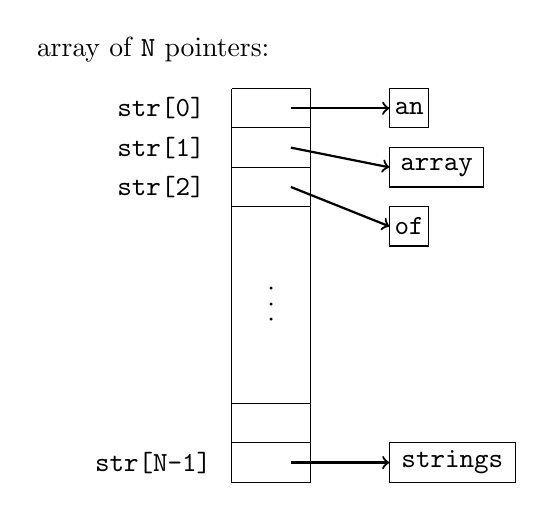
\begin{tikzpicture}
    \node at(0, 0.5) {array of \verb'N' pointers:};
    \draw (1, 0) -- (1, -5) -- (2, -5) -- (2, 0) -- (1, 0);
    \draw (1, -0.5) -- (2, -0.5);
    \draw (1, -1) -- (2, -1);
    \draw (1, -1.5) -- (2, -1.5);
    \draw (1, -4) -- (2, -4);
    \draw (1, -4.5) -- (2, -4.5);
    \node at(0.1, -0.25) {\verb'str[0]'};
    \node at(0.1, -0.75) {\verb'str[1]'};
    \node at(0.1, -1.25) {\verb'str[2]'};
    \node at(0, -4.75) {\verb'str[N-1]'};
    \draw[thick, ->] (1.75, -0.25) -- (3, -0.25);
    \node at(3.25, -0.25) {\verb'an'};
    \draw (3, 0) -- (3, -0.5) -- (3.5, -0.5) -- (3.5, 0) -- (3, 0);
    \draw[thick, ->] (1.75, -0.75) -- (3, -1);
    \node at(3.6, -1) {\verb'array'};
    \draw (3, -0.75) -- (3, -1.25) -- (4.2, -1.25) -- (4.2, -0.75) -- (3,
        -0.75);
    \draw[thick, ->] (1.75, -1.25) -- (3, -1.75);
    \node at(3.25, -1.75) {\verb'of'};
    \draw (3, -1.5) -- (3, -2) -- (3.5, -2) -- (3.5, -1.5) -- (3, -1.5);
    \draw[thick, ->] (1.75, -4.75) -- (3, -4.75);
    \node at(3.8, -4.75) {\verb'strings'};
    \draw (3, -4.5) -- (3, -5) -- (4.6, -5) -- (4.6, -4.5) -- (3, -4.5);
    \node at(1.5, -2.75) {$\cdot$};
    \node at(1.5, -2.55) {$\cdot$};
    \node at(1.5, -2.95) {$\cdot$};
    \end{tikzpicture}
\end{figure}\\
To sort elements \verb'str[0]' through \verb'str[N-1]' of an array of
strings, \verb'qsort' must be called with the array, its length, the size
of the items being sorted, and the comparison function:
\begin{wellcode}
    char *str[N];
    qsort(str, N, sizeof(str[0]), scmp);
\end{wellcode}

Here's a similar function \verb'icmp' for comparing integers:
\begin{wellcode}
    /* icmp: integer compare of *p1 and *p2 */
    int icmp(const void *p1, const void *p2)
    {
        int v1, v2;
        v1 = *(int *) p1;
        v2 = *(int *) p2;
        if (v1 < v2)
            return -1;
        else if (v1 == v2)
            return 0;
        else
            return 1;
    }
\end{wellcode}
We could write
\begin{badcode}
    return v1 - v2;
\end{badcode}
but if \verb'v2' is large and positive and \verb'v1' is large and negative
or vice versa (反过来), the resulting overflow would produce an incorrect
answer. Direct comparison is longer but safe.

Again, the call to \verb'qsort' requires the array, its length, the size of
the items being sorted, and the comparison function:
\begin{wellcode}
    int arr[N];
    qsort(arr, N, sizeof(arr[0]), icmp);
\end{wellcode}

ANSI C also defines a binary search routine, \verb'bsearch'. Like
\verb'qsort', \verb'bsearch' requires a pointer to a comparison function
(often the same one used for \verb'qsort'); it returns a pointer to the
matching element or \verb'NULL' if not found. Here is our HTML
\verb'lookup' routine, rewritten to use \verb'bsearch'
% "return np - tab" should be "return (np - tab)/sizeof(*tab)"?
\begin{wellcode}
    /* lookup: use bsearch to find name in tab, return index */
    int lookup(char *name, Nameval tab[], int ntab)
    {
        Nameval key, *np;
        key.name = name;
        key.value = 0;  /* unused; anything will do*/
        np = (Nameval *)bsearch(&key, tab, ntab, sizeof(tab[0]), nvcmp);
        if(np == NULL)
            return -1;
        else
            return np - tab;
    }
\end{wellcode}

As with \verb'qsort', the comparison routine receives the address of the
items to be compared, so the key must have that type; in this example, we
need to construct a fake \verb'Nameval' entry that is passed to the
comparison routine. The comparison routine itself is a function
\verb'nvcmp' that compares two \verb'Nameval' items by calling
\verb'strcmp' on their string components, ignoring their values:
\begin{wellcode}
    /* nvcmp: compare two Nameval names */
    int nvcmp(const void *va, const void *vb)
    {
        const Nameval *a, *b;
        a = (Nameval *)va;
        b = (Nameval *)vb;
        return strcmp(a->name, b->name);
    }
\end{wellcode}
This is analogous (相似) to \verb'scmp' but differs because the strings are
stored as members of a structure.

The clumsiness(笨拙) of providing the key means that \verb'bsearch'
provides less leverage(杠杆作用) than \verb'qsort'. A good general-purpose
sort routine takes a page or two of code, while binary search is not much
longer than the code it takes to interface to \verb'bsearch'. Nevertheless,
it's a good idea to use \verb'bsearch' instead of writing your own. Over
the years, binary search has proven surprisingly hard for programmers to
get right.

The standard C++ library has a generic algorithm called \verb'sort' that
guarantees $O(n\log n)$ behavior. The code is easier because it needs no
casts or element sizes, and it does not require an explicit comparison
function for types that have an order relation.
\begin{wellcode}
    int arr[N];
    sort(arr, arr + N);
\end{wellcode}
The C++ library also has generic binary search routines, with similar
notational (记数的) advantages.

\begin{exercise}
Quicksort is most naturally expressed recursively. Write it iteratively and
compare the two versions. (Hoare describes how hard it was to work out
quicksort iteratively, and how neatly (整洁地) it fell into place when he
did it recursively.)
\end{exercise}

\section{A Java Quicksort}
\label{sec:a_java_quicksort}

The situation in Java is different. Early releases had no standard sort
function, so we needed to write our own. More recent versions do provide a
sort function, however, which operates on classes that implement the
\verb'Comparable' interface, so we can now ask the library to sort for us.
But since the techniques are useful in other situations, in this section we
will work through the details of implementing quicksort in Java.

It's easy to adapt a quicksort for each type we might want to sort, but it
is more instructive to write a generic sort that can be called for any kind
of object, more in the style of the qsort interface.

One big difference from C or C++ that in Java it is not possible to pass a
comparison function to another function; there are no function pointers.
Instead we create an \textit{interface} whose sole (仅有的) content is a
function that compares two Objects. For each data type to be sorted, we
then create a class with a member function that implements the interface
for that data type. We pass an instance of that class to the sort function,
which in turn uses the comparison function within the class to compare
elements.

We begin by defining an interface named \verb'Cmp' that declares a single
member, a comparison function \verb'cmp' that compares two \verb'Objects':
\begin{wellcode}
    interface Cmp {
        int cmp(Object x, Object y);
    }
\end{wellcode}
Then we can write comparison functions that implement this interface; for
example, this class defines a function that compares \verb'Integer's:
\begin{wellcode}
    // Icmp: Integer comparison
    class Icmp implements Cmp {
        public int cmp(Object o1, Object o2)
        {
            int i1 = ((Integer) o1).intValue();
            int i2 = ((Integer) o2).intValue();
            if (i1 < i2)
                return -1;
            else if (i1 == i2)
                return 0;
            else
                return 1;
        }
    }
\end{wellcode}
and this compares \verb'Strings':
\begin{wellcode}
    // Scmp: String comparison
    class Scmp implements Cmp {
        public int cmp(Object o1, Object o2)
        {
            String s1 = (String) o1;
            String s2 = (String) o2;
            return s1.compareTo(s2);
        }
    }
\end{wellcode}
We can sort only types that are derived from \verb'Object' with this
mechanism; it cannot be applied to the basic types like \verb'int' or
\verb'double'. This is why we sort \verb'Integer's rather than \verb'int's.

With these components, we can now translate the C \verb'quicksort' function
into Java and have it call the comparison function from a \verb'Cmp' object
passed in as an argument. The most significant change is the use of indices
\verb'left' and \verb'right', since Java does not have pointers into
arrays.
\begin{wellcode}
    // Quicksort.sort: quicksort v[left]...v[right]
    static void sort(Object[] v, int left, int right, Cmp cmp)
    {
        int i, last;
        if (left >= right)  //nothing to do
            return;
        swap(v, left, rand(left, right));    // move pivot elem
        last = left;                        //      to v[left]
        for (i = left + 1; i <= right; i++) // partition
            if (cmp.cmp(v[i], v[left]) < 0)
                swap(v, ++last, i);
        swap(v, left, last);                // restore pivot elem
        sort(v, left, last - 1, cmp);       // recursively sort
        sort(v, last + 1, right, cmp);      //      each part
    }
\end{wellcode}
\verb'Quicksort.sort' uses \verb'cmp' to compare a pair of objects, and
calls \verb'swap' as before to interchange them.
\begin{wellcode}
    // Quicksort.swap: swap v[i] and v[j]
    static void swap(Object[] v, int i, int j)
    {
        Object temp;
        temp = v[i];
        v[i] = v[j];
        v[j] = temp;
    }
\end{wellcode}
Random number generation is done by a function that produces a random
integer in the range \verb'left' to \verb'right' inclusive:
\begin{wellcode}
    static Random rgen = new Random();

    // Quicksort.rand: return random integer in [left, right]
    static int rand(int left, int right)
    {
        return left + Math.abs(rgen.nextInt()) % (right - left + 1);
    }
\end{wellcode}
We compute the absolute value, using \verb'Math.abs', because Java's random
number generator returns negative integers as well as positive.

The functions \verb'sort', \verb'swap', and \verb'rand', and the generator
object \verb'rgen' are the members of a class \verb'Quicksort'.

Finally, to call \verb'Quicksort.sort' to sort a \verb'String' array, we
would say
\begin{wellcode}
    String[] sarr = new String[n];
    //fill n elements of sarr...
    Quicksort.sort(sarr, 0, sarr.length - 1, new Scmp());
\end{wellcode}
This calls \verb'sort' with a string-comparison object created for the
occasion.

\begin{exercise}
Our Java quicksort does a fair amount of type conversion as items are cast
from their original type (like \verb'Integer') to \verb'Object' and back
again.  Experiment with a version of \verb'Quicksort.sort' that uses the
specific type being sorted, to estimate what performance penalty is
incurred (蒙受) by type conversions.
\end{exercise}

\section{O-Notation}
\label{sec:o_notation}

We've described the amount of work to be done by a particular algorithm in
terms of $n$, the number of elements in the input. Searching unsorted data
can take time proportional to $n$; if we use binary search on sorted data,
the time will be proportional to $\log n$. Sorting times might be
proportional to $n^2$ or $n\log n$.

We need a way to make such statements more precise, while at the same time
abstracting away details like the CPU speed and the quality of the compiler
(and the programmer). We want to compare running times and space
requirements of algorithms independently of programming language, compiler,
machine architecture, processor speed, system load, and other complicating
factors.

There is a standard notation for this idea, called "O-notation". Its basic
parameter is $n$, the size of a problem instance, and the complexity or
running time is expressed as a function of $n$. The $"O"$ is for order
(阶数), as in "Binary search is $O(\log n)$; it takes on the order of $\log
n$ steps to search an array of $n$ items." The notation $O(f(n))$ means
that, once $n$ gets large, the running time is proportional to at most
$f(n)$, for example, $O(n^2)$ or $O(n\log n)$. Asymptotic (渐近的)
estimates like this are valuable for theoretical analyses and very helpful
for gross (总的) comparisons of algorithms, but details may make a
difference in practice. For example, a low-overhead $O(n^2)$ algorithm may
run faster than a high-overhead $O(n\log n)$ algorithm for small values of
$n$, but inevitably (必然地), if $n$ gets large enough, the algorithm with
the slower-growing functional behavior will be faster.

We must also distinguish between \term{worst-case} and \term{expected}
behavior. It's hard to define "expected," since it depends on assumptions
about what kinds of inputs will be given. We can usually be precise about
the worst case, although that may be misleading.  Quicksort's worst-case
run-time is $O(n^2)$ but the expected time is $O(n\log n)$. By choosing the
pivot element carefully each time, we can reduce the probability of
quadratic (二次的) or $O(n^2)$ behavior to essentially zero; in practice, a
well-implemented quicksort usually runs in $O(n\log n)$ time.

These are the most important cases:
\begin{center}
\begin{tabular}{lll}
Notation        & Name          & Example                   \\
\hline
$O(1)$          & constant      & array index               \\
$O(\log n)$     & logarithmic   & binary search             \\
$O(n)$          & linear        & string comparison         \\
$O(n\log n)$    & $n$log$n$     & quicksort                 \\
$O(n^2)$        & quadratic     & simple sorting methods    \\
$O(n^3)$        & cubic         & matrix multiplication     \\
$O(2^n)$        & exponential   & set partitioning
\end{tabular}
\end{center}

Accessing an item in an array is a constant-time or $O(1)$ operation. An
algorithm that eliminates half the input at each stage, like binary search,
will generally take $O(\log n)$. Comparing two $n$-character strings with
\verb'strcmp' is $O(n)$. The traditional matrix multiplication algorithm
takes $O(n^3)$, since each element of the output is the result of
multiplying $n$ pairs and adding them up, and there are $n^2$ elements in
each matrix.

Exponential-time algorithms are often the result of evaluating all
possibilities: there are $2^n$ subsets of a set of $n$ items, so an
algorithm that requires looking at all subsets will be exponential or
$O(2^n)$. Exponential algorithms are generally too expensive unless $n$ is
very small, since adding one item to the problem doubles the running time.
Unfortunately there are many problems, such as the famous "Traveling
Salesman Problem (货郎担问题)", for which only exponential algorithms are
known. When that is the case, algorithms that find approximations (近似) to
the best answer are often substituted (替代).

\begin{exercise}
What are some input sequences that might cause a quicksort implementation
to display worst-case behavior? Try to find some that provoke (引起) your
library version into running slowly. Automate the process so that you can
specify and perform a large number of experiments easily.
\end{exercise}

\begin{exercise}
Design and implement an algorithm that will sort an array of $n$ integers
as slowly as possible. You have to play fair: the algorithm must make
progress and eventually terminate, and the implementation must not cheat
with tricks like time-wasting loops. What is the complexity of your
algorithm as a function of $n$?
\end{exercise}

\section{Growing Arrays}
\label{sec:growing_arrays}

The arrays used in the past few sections have been static, with their size
and contents fixed at compile time. If the flabby (松驰的) word or HTML
character tables were to be modified at run-time, a hash table would be a
more appropriate data structure. Growing a sorted array by inserting $n$
elements one at a time is an $O(n^2)$ operation that should be avoided if
$n$ is large.

Often, though, we need to keep track of a variable but small number of
things, and arrays can still be the method of choice. To minimize the cost
of allocation, the array should be resized in chunks, and for cleanliness
the array should be gathered together with the information necessary to
maintain it. In C++ or Java, this would be done with classes from standard
libraries; in C, we can achieve a similar result with a \verb'struct'.

The following code defines a growable array of \verb'Nameval'
items; new items are added at the end of the array, which is grown as
necessary to make room. Any element can be accessed through its subscript
in constant time. This is analogous to the vector classes in the Java and
C++ libraries.
\begin{wellcode}
    typedef struct Nameval Nameval;
    struct Nameval {
        char *name;
        int value;
    };

    struct NVtab {
        int nval;       /* current number of values */
        int max;        /* allocated number of values */
        Nameval *nameval;   /* array of name-value pairs */
    } nvtab;

    enum { NVINIT = 1, NVGROW = 2 };

    /* addname: add new name and value to nvtab */
    int addname (Nameval newname)
    {
        Nameval *nvp;
        if (nvtab.nameval == NULL) {    /* first time */
            nvtab.nameval =
                (Nameval *)malloc(NVINIT * sizeof(Nameval));
            if (nvtab.nameval == NULL)
                return -1;
            nvtab.max = NVINIT;
            nvtab.nval = 0;
        }
        else if (nvtab.nval >= nvtab.max) { /* grow */
            nvp = (Nameval *) realloc(nvtab.nameval,
                        (NVGROW * nvtab.max) * sizeof(Nameval));
            if (nvp == NULL)
                return -1;
            nvtab.max *= NVGROW;
            nvtab.nameval = nvp;
        }
        nvtab.nameval[nvtab.nval] = newname;
        return nvtab.nval++;
    }
\end{wellcode}
The function \verb'addname' returns the index of the item just added, or
\verb'-1' if some error occurred.

The call to \verb'realloc' grows the array to the new size, preserving the
existing elements, and returns a pointer to it or \verb'NULL' if there
isn't enough memory. Doubling the size in each \verb'realloc' keeps the
expected cost of copying each element constant: if the array grew by just
one element on each call, the performance could be $O(n^2)$. Since the
address of the array may change when it is reallocated, the rest of the
program must refer to elements of the array by subscripts, not pointers.
Note that the code doesn't say
\begin{badcode}
    nvtab.nameval = (Nameval *) realloc(nvtab.nameval,
            (NVGROW * nvtab.max) * sizeof(Nameval));
\end{badcode}
In this form, if the reallocation were to fail, the original array would be
lost.

We start with a very small initial value (\verb'NVINIT = 1') for the array
size.  This forces the program to grow its arrays right away and thus
ensures that this part of the program is exercised. The initial size can be
increased once the code goes into production use, though the cost of
starting small is negligible (可以忽略的).

The return value of \verb'realloc' does not need to be cast to its final
type because C promotes (提升) the \verb'void *' automatically. But C++
does not; there the cast is required. One can argue about whether it is
safer to cast (cleanliness, honesty) or not to cast (the cast can hide
genuine (真正的) errors).  We chose to cast because it makes the program
legal in both C and C++; the price is less error-checking from the C
compiler, but that is offset by the extra checking available from using two
compilers.

Deleting a name can be tricky, because we must decide what to do with the
resulting gap in the array. If the order of elements does not matter, it is
easiest to swap the last element into the hole. If order is to be
preserved, however, we must move the elements beyond the hole down by one
position:
\begin{wellcode}
    /* delname: remove first matching nameval from nvtab */
    int delname(char *name)
    {
        int i;
        for (i = 0; i < nvtab.nval; i++)
            if (strcmp(nvtab.nameval[i].name, name) == 0) {
                memmove(nvtab.nameval + i, nvtab.nameval + i + 1,
                             (nvtab.nval - (i + 1)) * sizeof(Nameval));
                nvtab.nval--;
                return 1;
            }
        return 0;
    }
\end{wellcode}
The call to \verb'memmove' squeezes the array by moving the elements down
one position; \verb'memmove' is a standard library routine for copying
arbitrary-sized blocks of memory.

The ANSI C standard defines two functions: \verb'memcpy', which is fast but
might overwrite memory if source and destination overlap; and
\verb'memmove', which might be slower but will always be correct. The
burden of choosing correctness over speed should not be placed upon the
programmer; there should be only one function. Pretend there is, and always
use \verb'memmove'.

We could replace the \verb'memmove' call with the following loop:
\begin{wellcode}
    int j;
    for (j = i; j < nvtab.nval - 1; j++)
        nvtab.nameval[j] = nvtab.nameval[j + 1];
\end{wellcode}
We prefer to use \verb'memmove' because it avoids the easy-to-make mistake
of copying the elements in the wrong order. If we were inserting instead of
deleting, the loop would need to count down, not up, to avoid overwriting
elements. By calling \verb'memmove' we don't need to think it through each
time.

An alternative to moving the elements of the array is to mark deleted
elements as unused. Then to add a new item, first search for an unused slot
and grow the vector only if none is found. In this example, an element can
be marked as unused by setting its name field to \verb'NULL'.

Arrays are the simplest way to group data; it's no accident that most
languages provide efficient and convenient indexed arrays and represent
strings as arrays of characters. Arrays are easy to use, provide $O(1)$
access to any item, work well with binary search and quicksort, and have
little space overhead. For fixed-size data sets, which can even be
constructed at compile time, or for guaranteed small collections of data,
arrays are unbeatable. But maintaining a changing set of values in an array
can be expensive, so if the number of elements is unpredictable and
potentially large, it may be better to use another data structure.

\begin{exercise}
    In the code above, \verb'delname' doesn't call \verb'realloc' to return
    (归还) the memory freed by the deletion. Is this worthwhile? How would
    you decide whether to do so?
\end{exercise}

\begin{exercise}
Implement the necessary changes to \verb'addname' and \verb'delname' to
delete items by marking deleted items as unused. How isolated is the rest
of the program from this change?
\end{exercise}

\section{Lists}
\label{sec:lists}

Next to arrays, lists are the most common data structure in typical
programs. Many languages have built-in list types -- some, such as Lisp,
are based on them -- but in C we must build them ourselves. In C++ and
Java, lists are implemented by a library, but we still need to know how and
when to use it. In this section we're going to discuss lists in C but the
lessons apply more broadly.

A \emph{singly-linked list} is a set of items, each with data
and a pointer to the next item. The head of the list is a pointer to the
first item and the end of the list is marked by a null pointer. This shows
a list with four elements:
\begin{center}
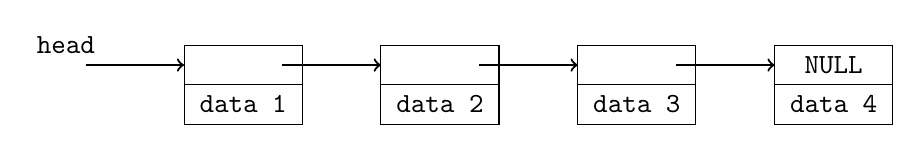
\begin{tikzpicture}
\node at(0, 0) {\texttt{head}};
\draw (1.5, 0) -- (1.5, -1) -- (3, -1) -- (3, 0) -- (1.5, 0);
\draw (4, 0) -- (4, -1) -- (5.5, -1) -- (5.5, 0) -- (4, 0);
\draw (6.5, 0) -- (6.5, -1) -- (8, -1) -- (8, 0) -- (6.5, 0);
\draw (9, 0) -- (9, -1) -- (10.5, -1) -- (10.5, 0) -- (9, 0);
\draw (1.5, -0.5) -- (3, -0.5);
\draw (4, -0.5) -- (5.5, -0.5);
\draw (6.5, -0.5) -- (8, -0.5);
\draw (9, -0.5) -- (10.5, -0.5);
\draw[thick, ->] (0.25, -0.25) -- (1.5, -0.25);
\draw[thick, ->] (2.75, -0.25) -- (4, -0.25);
\draw[thick, ->] (5.25, -0.25) -- (6.5, -0.25);
\draw[thick, ->] (7.75, -0.25) -- (9, -0.25);
\node at(2.25, -0.75) {\texttt{data 1}};
\node at(4.75, -0.75) {\texttt{data 2}};
\node at(7.25, -0.75) {\texttt{data 3}};
\node at(9.75, -0.75) {\texttt{data 4}};
\node at(9.75, -0.25) {\texttt{NULL}};
\end{tikzpicture}
\end{center}
There are several important differences between arrays and lists. First,
arrays have fixed size but a list is always exactly the size it needs to be
to hold its contents, plus some per-item storage overhead to hold the
pointers. Second, lists can be rearranged by exchanging a few pointers,
which is cheaper than the block move necessary in an array. Finally, when
items are inserted or deleted the other items aren't moved; if we store
pointers to the elements in some other data structure, they won't be
invalidated by changes to the list.

These differences suggest that if the set of items will change frequently,
particularly if the number of items is unpredictable, a list is the way to
store them; by comparison, an array is better for relatively static data.

There are a handful of fundamental list operations: add a new item to the
front or back, find a specific item, add a new item before or after a
specific item, and perhaps delete an item. The simplicity of lists makes it
easy to add other operations as appropriate.

Rather than defining an explicit \verb'List' type, the usual way lists are
used in C is to start with a type for the elements, such as our HTML
\verb'Nameval', and add a pointer that links to the next element:
\begin{wellcode}
    typedef struct Nameval Nameval;
    struct Nameval {
        char *name;
        int value;
        Nameval *next; /* in list */
    };
\end{wellcode}
It's difficult to initialize a non-empty list at compile time, so, unlike
arrays, lists are constructed dynamically. First, we need a way to
construct an item. The most direct approach is to allocate one with a
suitable function, which we call \verb'newitem':
\begin{wellcode}
    /* newitem: create new item from name and value */
    Nameval *newitem(char *name, int value)
    {
        Nameval *newp;
        newp = (Nameval *) emalloc(sizeof(Nameval));
        newp->name = name;
        newp->value = value;
        newp->next = NULL;
        return newp;
    }
\end{wellcode}
The routine \verb'emalloc' is one we'll use throughout the book; it calls
\verb'malloc', and if the allocation fails, it reports the error and exits
the program. We'll show the code in Chapter \ref{chap:interface}; for now,
it's sufficient to regard \verb'emalloc' as a memory allocator that never
returns failure.

The simplest and fastest way to assemble a list is to add each new element
to the front:
\begin{wellcode}
    /* addfront: add newp to front of listp */
    Nameval *addfront(Nameval *listp, Nameval *newp)
    {
        newp->next = listp;
        return newp;
    }
\end{wellcode}

When a list is modified, it may acquire a different first element, as it
does when \verb'addfront' is called. Functions that update a list must
return a pointer to the new first element, which is stored in the variable
that holds the list. The function \verb'addfront' and other functions in
this group all return the pointer to the first element as their function
value; a typical use is
\begin{wellcode}
    nvlist = addfront(nvlist, newitem("smiley", 0x263A));
\end{wellcode}
This design works even if the existing list is empty (null) and makes it
easy to combine the functions in expressions. It seems more natural than
the alternative of passing in a pointer to the pointer holding the head of
the list.

Adding an item to the end of a list is an $O(n)$ procedure, since we must
walk the list to find the end:
\begin{wellcode}
    /* addend: add newp to end of listp */
    Nameval *addend(Nameval *listp, Nameval *newp)
    {
        Nameval *p;
        if (listp == NULL)
            return newp;
        for (p = listp; p->next != NULL; p = p->next)
            ;
        p->next = newp;
        return listp;
    }
\end{wellcode}
If we want to make \verb'addend' an $O(1)$ operation, we can keep a
separate pointer to the end of the list. The drawback to this approach,
besides the bother of maintaining the end pointer, is that a list is no
longer represented by a single pointer variable. We'll stick with the
simple style.

To search for an item with a specific name, follow the \verb'next'
pointers:
\begin{wellcode}
    /* lookup: sequential search for name in listp */
    Nameval *lookup(Nameval *listp, char *name)
    {
        for (; listp != NULL; listp = listp->next)
            if (strcmp(name, listp->name) == 0)
                return listp ;
        return NULL; /* no match */
    }
\end{wellcode}
This takes $O(n)$ time and there's no way to improve that bound in general.
Even if the list is sorted, we need to walk along the list to get to a
particular element. Binary search does not apply to lists.

To print the elements of a list, we can write a function to walk the list
and print each element; to compute the length of a list, we can write a
function to walk the list and increment a counter; and so on. An
alternative is to write one function, \verb'apply', that walks a list and
calls another function for each list element. We can make \verb'apply' more
flexible by providing it with an argument to be passed each time it calls
the function. So \verb'apply' has three arguments: the list, a function to
be applied to each element of the list, and an argument for that function:
\begin{wellcode}
    /* apply: execute fn for each element of listp*/
    void apply(Nameval *listp,
            void (*fn)(Nameval *, void *), void *arg)
    {
        for (; listp != NULL; listp = listp->next)
            (*fn)(listp, arg);      /* call the function */
    }
\end{wellcode}
The second argument of \verb'apply' is a pointer to a function that takes
two arguments and returns \verb'void'. The standard but awkward syntax,
\begin{wellcode}
    void (*fn)(Nameval*, void*)
\end{wellcode}
declares \verb'fn' to be a pointer to a \verb'void'-valued function, that
is, a variable that holds the address of a function that returns
\verb'void'. The function takes two arguments, a \verb'Nameval *', which is
the list element, and a \verb'void *', which is a generic pointer to an
argument for the function.

To use \verb'apply', for example to print the elements of a list, we could
write a trivial function whose argument is a format string:
\begin{wellcode}
    /* printnv: print name and value using format in arg */
    void printnv(Nameval *p, void *arg)
    {
        char *fmt;
        fmt = (char*)arg;
        printf(fmt, p->name, p->value);
    }
\end{wellcode}
which we call like this:
\begin{wellcode}
    apply(nvlist, printnv, "%s: %x\n");
\end{wellcode}
To count the elements, we define a function whose argument is a pointer to
an integer to be incremented:
\begin{wellcode}
    /* inccounter: increment counter *arg */
    void inccounter(Nameval *p, void *arg)
    {
        int *ip;
        /* p is unused */
        ip = (int *) arg;
        (*ip)++;
    }
\end{wellcode}
and call it like this:
\begin{wellcode}
    int n;
    n = 0;
    apply(nvlist, inccounter, &n);
    printf("%d elements in nvlist\n", n);
\end{wellcode}

Not every list operation is best done this way. For instance, to destroy a
list we must use more care:
\begin{wellcode}
    /* freeall: free all elements of listp */
    void freeall(Nameval *listp)
    {
        Nameval *next;
        for (; listp != NULL; listp = next) {
            next = listp->next;
            /* assumes name is freed elsewhere */
            free(listp);
        }
    }
\end{wellcode}
Memory cannot be used after it has been freed, so we must save
\verb'listp->next' in a local variable, called \verb'next', before freeing
the element pointed to by \verb'listp'. If the loop read, like the others,
\begin{badcode}
    for (; listp != NULL; listp = listp->next)
        free(listp);
\end{badcode}
the value of \verb'listp->next' could be overwritten by \verb'free' and the
code would fail.

Notice that \verb'freeall' does not free \verb'listp->name'. It assumes
that the \verb'name' field of each \verb'Nameval' will be freed somewhere
else, or was never allocated. Making sure items are allocated and freed
consistently requires agreement between \verb'newitem' and \verb'freeall';
there is a tradeoff between guaranteeing that memory gets freed
and making sure things aren't freed that shouldn't be. Bugs are frequent
when this is done wrong. In other languages, including Java, garbage
collection solves this problem for you. We will return to the topic of
resource management in Chapter \ref{chap:interface}. Deleting a single
element from a list is more work than adding one:
\begin{wellcode}
    /* delitem: delete first "name" from listp */
    Nameval *delitem(Nameval *listp, char *name)
    {
        Nameval *p, *prev;
        prev = NULL;
        for (p = listp; p != NULL; p = p->next) {
            if (strcmp(name, p->name) == 0) {
                if (prev == NULL)
                    listp = p->next;
                else
                    prev->next = p->next;
                free(p);
                return listp;
            }
            prev = p;
        }
        eprintf("delitem: %s not in list", name);
        return NULL;    /* can't get here */
    }
\end{wellcode}
As in \verb'freeall', \verb'delitem' does not free the \verb'name' field.

The function \verb'eprintf' displays an error message and exits the
program, which is clumsy (笨拙的) at best. Recovering gracefully from
errors can be difficult and requires a longer discussion that we defer to
Chapter \ref{chap:interface}, where we will also show the implementation of
\verb'eprintf'.

These basic list structures and operations account for the vast majority of
applications that you are likely to write in ordinary programs. But there
are many alternatives. Some libraries, including the C++ Standard Template
Library, support doubly-linked lists, in which each element has two
pointers, one to its successor and one to its predecessor. Doubly-linked
lists require more overhead, but finding the last element and deleting the
current element are $O(1)$ operations. Some allocate the list pointers
separately from the data they link together; these are a little harder to
use but permit items to appear on more than one list at the same time.

Besides being suitable for situations where there are insertions and
deletions in the middle, lists are good for managing unordered data of
fluctuating (波动的) size, especially when access tends to be
last-in-first-out (LIFO), as in a stack. They make more effective use of
memory than arrays do when there are multiple stacks that grow and shrink
independently. They also behave well when the information is ordered
intrinsically (本质地) as a chain of a unknown \term{priori} (先验) size,
such as the successive words of a document. If you must combine frequent
update with random access, however, it would be wiser to use a less
insistently (执着地) linear data structure, such as a tree or hash table.

\begin{exercise}
Implement some of the other list operators: copy, merge, split, insert
before or after a specific item. How do the two insertion operations differ
in difficulty? How much can you use the routines we've written, and how
much must you create yourself?
\end{exercise}

\begin{exercise}
Write recursive and iterative versions of \verb'reverse', which reverses a
list.  Do not create new list items: re-use the existing ones.
\end{exercise}

\begin{exercise}
Write a generic List type for C. The easiest way is to have each list item
hold a \verb'void *', that points to the data. Do the same for C++ by
defining a template and for Java by defining a class that holds lists of
type Object. What are the strengths and weaknesses of the various languages
for this job?
\end{exercise}

\begin{exercise}
    Devise (设计) and implement a set of tests for verifying that the list
    routines you write are correct. Chapter \ref{chap:testing} discusses
    strategies for testing.
\end{exercise}

\section{Trees}
\label{sec:trees}

A tree is a hierarchical data structure that stores a set of items in which
each item has a value, may point to zero or more others, and is pointed to
by exactly one other. The \term{root} of the tree is the sole
exception; no item points to it.

There are many types of trees that reflect complex structures, such as
parse trees that capture the syntax of a sentence or a program, or family
trees that describe relationships among people. We will illustrate the
principles with binary search trees, which have two links at each node.
They're the easiest to implement, and demonstrate the essential properties
of trees. A node in a binary search tree has a value and two pointers,
\verb'left' and \verb'right', that point to its children. The child
pointers may be null if the node has fewer than two children. In a binary
search tree, the values at the nodes define the tree: all children to the
left of a particular node have lower values, and all children to the right
have higher values. Because of this property, we can use a variant of
binary search to search the tree quickly for a specific value or determine
that it is not present.

The tree version of \verb'Nameval' is straightforward:
\begin{wellcode}
    typedef struct Nameval Nameval;
    struct Nameval {
        char *name;
        int value;
        Nameval *left;  /* lesser */
        Nameval *right; /* greater */
    };
\end{wellcode}
The \textit{lesser} and \textit{greater} comments refer to the properties
of the links: left children store lesser values, right children store
greater values.

As a concrete example, this figure shows a subset of a character name table
stored as a binary search tree of \verb'Nameval's, sorted by ASCII
character values in the names:
\begin{center}
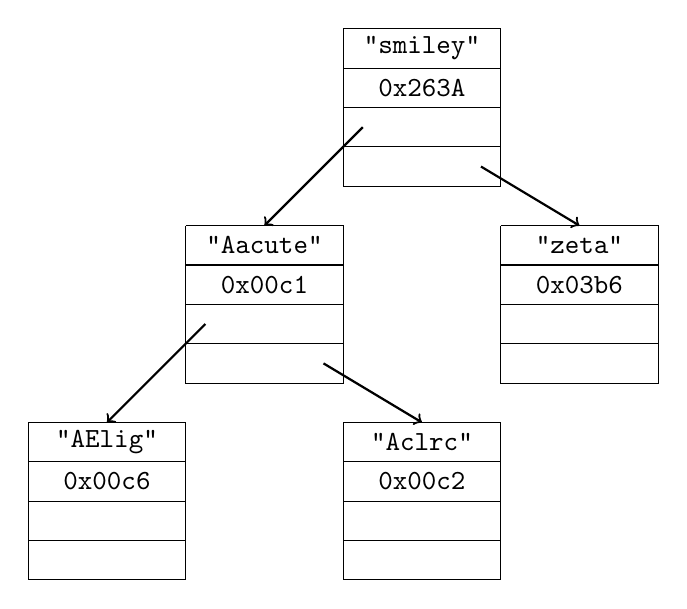
\begin{tikzpicture}
    \draw (4, 0) -- (4, -2) -- (6, -2) -- (6, 0) -- (4, 0);
    \draw (4, -0.5) -- (6, -0.5);
    \draw (4, -1) -- (6, -1);
    \draw (4, -1.5) -- (6, -1.5);
    \node at (5, -0.25) {\texttt{"smiley"}};
    \node at (5, -0.75) {\texttt{0x263A}};
    \draw (2, -2.5) -- (2, -4.5) -- (4, -4.5) -- (4, -2.5) -- (2, -2.5);
    \draw (2, -3) -- (4, -3);
    \draw (2, -3.5) -- (4, -3.5);
    \draw (2, -4) -- (4, -4);
    \node at (3, -2.75) {\texttt{"Aacute"}};
    \node at (3, -3.25) {\texttt{0x00c1}};
    \draw (6, -2.5) -- (6, -4.5) -- (8, -4.5) -- (8, -2.5) -- (6, -2.5);
    \draw (6, -3) -- (8, -3);
    \draw (6, -3.5) -- (8, -3.5);
    \draw (6, -4) -- (8, -4);
    \node at (7, -2.75) {\texttt{"zeta"}};
    \node at (7, -3.25) {\texttt{0x03b6}};
    \draw (0, -5) -- (0, -7) -- (2, -7) -- (2, -5) -- (0, -5);
    \draw (0, -5.5) -- (2, -5.5);
    \draw (0, -6) -- (2, -6);
    \draw (0, -6.5) -- (2, -6.5);
    \node at (1, -5.25) {\texttt{"AElig"}};
    \node at (1, -5.75) {\texttt{0x00c6}};
    \draw (4, -5) -- (4, -7) -- (6, -7) -- (6, -5) -- (4, -5);
    \draw (4, -5.5) -- (6, -5.5);
    \draw (4, -6) -- (6, -6);
    \draw (4, -6.5) -- (6, -6.5);
    \node at (5, -5.25) {\texttt{"Aclrc"}};
    \node at (5, -5.75) {\texttt{0x00c2}};
    \draw[thick, ->] (4.25, -1.25) -- (3, -2.5);
    \draw[thick, ->] (5.75, -1.75) -- (7, -2.5);
    \draw[thick, ->] (2.25, -3.75) -- (1, -5);
    \draw[thick, ->] (3.75, -4.25) -- (5, -5);
\end{tikzpicture}
\end{center}

With multiple pointers to other elements in each node of a tree, many
operations that take time $O(n)$ in lists or arrays require only $O(\log
n)$ time in trees. The multiple pointers at each node reduce the time
complexity of operations by reducing the number of nodes one must visit to
find an item.

A binary search tree (which we'll call just "tree" in this section) is
constructed by descending into the tree recursively, branching left or
right as appropriate, until we find the right place to link in the new
node, which must be a properly initialized object of type \verb'Nameval': a
name, a value, and two null pointers. The new node is added as a leaf, that
is, it has no children yet.
\begin{wellcode}
    /* insert: insert newp in treep, return treep */
    Nameval *insert(Nameval *treep, Nameval *newp)
    {
        int cmp;
        if (treep == NULL)
            return newp;
        cmp = strcmp(newp->name, treep->name);
        if (cmp == 0)
            weprintf("insert: duplicate entry %s ignored",
                    newp->name);
        else if (cmp < 0)
            treep->left = insert(treep->left, newp);
        else
            treep->right = insert(treep->right, newp);
        return treep;
    }
\end{wellcode}
We haven't said anything before about duplicate entries. This version of
\verb'insert' complains about attempts to insert duplicate entries
\verb'(cmp == 0)' in the tree. The list insert routine didn't complain
because that would require searching the list, making insertion $O(n)$
rather than $O(1)$. With trees, however, the test is essentially free and
the properties of the data structure are not as clearly defined if there
are duplicates. In other applications, though, it might be necessary to
accept duplicates, or it might be reasonable to ignore them completely.

The \verb'weprintf' routine is a variant of \verb'eprintf'; it prints an
error message, prefixed with the word \verb'warning', but unlike
\verb'eprintf' it does not terminate the program.

A tree in which each path from the root to a leaf has approximately the
same length is called balanced. The advantage of a balanced tree is that
searching it for an item is an $O(\log n)$ process, since, as in binary
search, the number of possibilities is halved at each step.

If items are inserted into a tree as they arrive, the tree might not be
balanced; in fact, it might be badly unbalanced. If the elements arrive
already sorted, for instance, the code will always descend down one branch
of the tree, producing in effect a list down the \verb'right' links, with
all the performance problems of a list. If the elements arrive in random
order, however, this is unlikely to happen and the tree will be more or
less balanced.

It is complicated to implement trees that are guaranteed to be balanced;
this is one reason there are many kinds of trees. For our purposes, we'll
just sidestep (回避) the issue and assume that incoming data is
sufficiently random to keep the tree balanced enough.

The code for \verb'lookup' is similar to \verb'insert':
\begin{wellcode}
    /* lookup: lookup name in tree treep */
    Nameval *lookup(Nameval *treep, char *name)
    {
        int cmp;
        if (treep == NULL)
            return NULL;
        cmp = strcmp(name, treep->name);
        if (cmp == 0)
            return treep;
        else if (cmp < 0)
            return lookup(treep->left, name);
        else
            return lookup(treep->right, name);
    }
\end{wellcode}

There are a couple of things to notice about \verb'lookup' and
\verb'insert'. First, they look remarkably like the binary search algorithm
at the beginning of the chapter. This is no accident, since they share an
idea with binary search: divide and conquer (分而治之), the origin of
logarithmic-time performance.

Second, these routines are recursive. If they are rewritten as iterative
algorithms they will be even more similar to binary search. In fact, the
iterative version of \verb'lookup' can be constructed by applying an
elegant transformation to the recursive version. Unless we have found the
item, \verb'lookup''s last action is to return the result of a call to
itself, a situation called \term{tail recursion}. This can be converted to
iteration by patching up (修补) the arguments and restarting the routine.
The most direct method is to use a \verb'goto' statement, but a
\verb'while' loop is cleaner:
\begin{wellcode}
    /* nrlookup: non-recursively lookup name in tree treep */
    Nameval *nrlookup(Nameval *treep, char *name)
    {
        int cmp;
        while (treep != NULL) {
            cmp = strcmp(name, treep->name);
            if (cmp == 0)
                return treep;
            else if (cmp < 0)
                treep = treep->left;
            else
                treep = treep->right;
        }
        return NULL;
    }
\end{wellcode}

Once we can walk the tree, the other common operations follow naturally. We
can use some of the techniques from list management, such as writing a
general tree-traverser that calls a function at each node. This time,
however, there is a choice to make: when do we perform the operation on
this item and when do we process the rest of the tree? The answer depends
on what the tree is representing; if it's storing data in order, such as a
binary search tree, we visit the left half before the right. Sometimes the
tree structure reflects some intrinsic (本质的) ordering of the data, such
as in a family tree, and the order in which we visit the leaves will depend
on the relationships the tree represents.

An \emph{in-order} traversal executes the operation after visiting the left
subtree and before visiting the right subtree:
\begin{wellcode}
    /* applyinorder: inorder application of fn to treep */
    void applyinorder(Nameval *treep,
            void (*fn)(Nameval *, void *), void *arg)
    {
        if (treep == NULL)
            return;
        applyinorder(treep->left, fn, arg);
        (*fn)(treep, arg);
        applyinorder(treep->right, fn, arg);
    }
\end{wellcode}
This sequence is used when nodes are to be processed in sorted order, for
example to print them all in order, which would be done as
\begin{wellcode}
    applyinorder(treep, printnv, "%s: %x\n");
\end{wellcode}
It also suggests a reasonable way to sort: insert items into a tree,
allocate an array of the right size, then use in-order traversal to store
them in the array in sequence.

A \term{post-order} traversal invokes the operation on the current node
after visiting the children:
\begin{wellcode}
    /* applypostorder: postorder application of fn to treep */
    void applypostorder(Nameval *treep,
            void (*fn)(Nameval *, void *), void *arg)
    {
        if (treep == NULL)
            return;;
        applypostorder(treep->left, fn, arg);
        applypostorder(treep->right, fn, arg);
        (*fn)(treep, arg);
    }
\end{wellcode}
Post-order traversal is used when the operation on the node depends
on the subtrees below it. Examples include computing the height of
a tree (take the maximum of the height of each of the two subtrees
and add one), laying out a tree in a graphics drawing package (allocate
space on the page for each subtree and combine them for this
node's space), and measuring total storage.

A third choice, \term{pre-order}, is rarely used so we'll omit (省略) it.

Realistically, binary search trees are infrequently used, though B-trees,
which have very high branching, are used to maintain information on
secondary storage. In day-to-day (日常) programming, one common use of a
tree is to represent the structure of a statement or expression. For
example, the statement
\begin{wellcode}
    mid = (low + high) / 2;
\end{wellcode}
can be represented by the \term{parse tree} shown in the figure
below. To evaluate the tree, do a post-order traversal and perform the
appropriate operation at each node.
\begin{center}
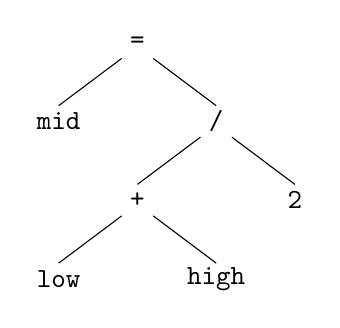
\begin{tikzpicture}
    \node at (1, 0) {\verb'='};
    \node at (0, -1) {\verb'mid'};
    \node at (2, -1) {\verb'/'};
    \node at (1, -2) {\verb'+'};
    \node at (3, -2) {\verb'2'};
    \node at (0, -3) {\verb'low'};
    \node at (2, -3) {\verb'high'};
    \draw (0.8, -0.2) -- (0, -0.8);
    \draw (1.2, -0.2) -- (2, -0.8);
    \draw (1.8, -1.2) -- (1, -1.8);
    \draw (2.2, -1.2) -- (3, -1.8);
    \draw (0.8, -2.2) -- (0, -2.8);
    \draw (1.2, -2.2) -- (2, -2.8);
\end{tikzpicture}
\end{center}
We'll take a longer look at parse trees in Chapter \ref{chap:notation}.

\begin{exercise}
Compare the performance of \verb'lookup' and \verb'nrlookup'. How expensive
is recursion compared to iteration?
\end{exercise}

\begin{exercise}
Use in-order traversal to create a sort routine. What time complexity does
it have? Under what conditions might it behave poorly? How does its
performance compare to our \verb'quicksort' and a library version?
\end{exercise}

\begin{exercise}
Devise and implement a set of tests for verifying that the tree routines
are correct.
\end{exercise}

\section{Hash Tables}
\label{sec:hash_tables}

Hash tables are one of the great inventions of computer science. They
combine arrays, lists, and some mathematics to create an efficient
structure for storing and retrieving dynamic data. The typical application
is a symbol table, which associates some value (the data) with each member
of a dynamic set of strings (the keys). Your favorite compiler almost
certainly uses a hash table to manage information about each variable in
your program. Your web browser may well use a hash table to keep track of
recently-used pages, and your connection to the Internet probably uses one
to cache recently-used domain names and their IP addresses.

The idea is to pass the key through a hash function to generate a hash
value that will be evenly distributed through a modest-sized integer range.
The hash value is used to index a table where the information is stored.
Java provides a standard interface to hash tables. In C and C++ the usual
style is to associate with each hash value (or "bucket") a list of the
items that share that hash, as this figure illustrates:
\begin{center}
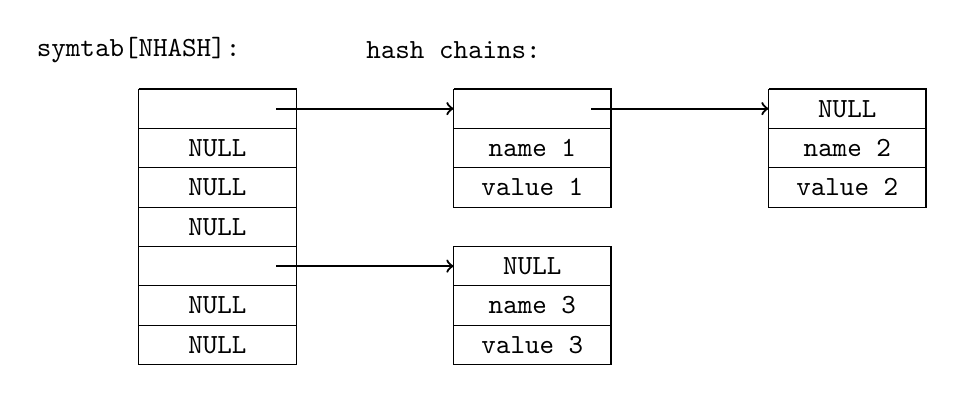
\begin{tikzpicture}
    \node at (0, 0) {\verb'symtab[NHASH]:'};
    \node at (4, 0) {\verb'hash chains:'};
    \draw (0, -0.5) -- (0, -4) -- (2, -4) -- (2, -0.5) -- (0, -0.5);
    \draw (0, -0.5) -- (2, -0.5);
    \draw (0, -1) -- (2, -1);
    \draw (0, -1.5) -- (2, -1.5);
    \draw (0, -2) -- (2, -2);
    \draw (0, -2.5) -- (2, -2.5);
    \draw (0, -3) -- (2, -3);
    \draw (0, -3.5) -- (2, -3.5);
    \node at (1, -3.75) {\verb'NULL'};
    \node at (1, -1.25) {\verb'NULL'};
    \node at (1, -1.75) {\verb'NULL'};
    \node at (1, -2.25) {\verb'NULL'};
    \node at (1, -3.25) {\verb'NULL'};
    \draw[thick, ->] (1.75, -0.75) -- (4, -0.75);
    \draw[thick, ->] (5.75, -0.75) -- (8, -0.75);
    \draw[thick, ->] (1.75, -2.75) -- (4, -2.75);
    \draw (4, -0.5) -- (4, -2) -- (6, -2) -- (6, -0.5) -- (4, -0.5);
    \draw (4, -1.5) -- (6, -1.5);
    \draw (4, -1) -- (6, -1);
    \node at (5, -1.25) {\verb'name 1'};
    \node at (5, -1.75) {\verb'value 1'};
    \draw (8, -0.5) -- (8, -2) -- (10, -2) -- (10, -0.5) -- (8, -0.5);
    \draw (8, -1.5) -- (10, -1.5);
    \draw (8, -1) -- (10, -1);
    \node at (9, -0.75) {\verb'NULL'};
    \node at (9, -1.25) {\verb'name 2'};
    \node at (9, -1.75) {\verb'value 2'};
    \draw (4, -2.5) -- (4, -4) -- (6, -4) -- (6, -2.5) -- (4, -2.5);
    \draw (4, -3) -- (6, -3);
    \draw (4, -3.5) -- (6, -3.5);
    \node at (5, -2.75) {\verb'NULL'};
    \node at (5, -3.25) {\verb'name 3'};
    \node at (5, -3.75) {\verb'value 3'};
\end{tikzpicture}
\end{center}
In practice, the hash function is pre-defined and an appropriate size of
array is allocated, often at compile time. Each element of the array is a
list that chains together the items that share a hash value. In other
words, a hash table of $n$ items is an array of lists whose average length
is $n/(array size)$. Retrieving an item is an $O(1)$ operation provided we
pick a good hash function and the lists don't grow too long.

Because a hash table is an array of lists, the element type is the same as
for a list:
\begin{wellcode}
    typedef struct Nameval Nameval;
    struct Nameval {
        char *name;
        int value;
        Nameval *next;      /* in chain */
    };
    Nameval *symtab[NHASH]; /* a symbol table */
\end{wellcode}

The list techniques we discussed in Section \ref{sec:lists} can be used to
maintain the individual hash chains. Once you've got a good hash function,
it's smooth sailing: just pick the hash bucket and walk along the list
looking for a perfect match. Here is the code for a hash table
\verb'lookup' / \verb'insert' routine. If the item is found, it is
returned.  If the item is not found and the \verb'create' flag is set,
\verb'lookup' adds the item to the table.  Again, this does not create a
copy of the name, assuming that the caller has made a safe copy instead.
\begin{wellcode}
    /* lookup: find name in symtab, with optional create */
    Nameval *lookup(char *name, int create, int value)
    {
        int h;
        Nameval *sym;
        h = hash(name);
        for (sym = symtab[h]; sym != NULL; sym = sym->next)
            if (strcmp(name, sym->name) == 0)
                return sym;
        if (create) {
            sym = (Nameval *)emalloc(sizeof(Nameval));
            sym->name = name;   /* assumed allocated elsewhere*/
            sym->value = value;
            sym->next = symtab[h];
            symtab[h] = sym;
        }
        return sym;
    }
\end{wellcode}
This combination of lookup and optional insertion is common. Without it,
there is duplication of effort; one must write 
\begin{wellcode}
    if (lookup("name") == NULL)
        additem(newitem("name", value));
\end{wellcode}
and the \verb'hash' is computed twice.

How big should the array be? The general idea is to make it big enough that
each hash chain will have at most a few elements, so that \verb'lookup' will be
$O(1)$. For instance, a compiler might have an array size of a few
thousand, since a large source file has a few thousand lines, and we don't
expect more than about one new identifier per line of code.

We must now decide what the hash function, \verb'hash', should calculate.
The function must be deterministic and should be fast and distribute the
data uniformly throughout the array. One of the most common hashing
algorithms for strings builds a hash value by adding each byte of the
string to a multiple of the hash so far. The multiplication spreads bits
from the new byte through the value so far; at the end of the loop, the
result should be a thorough mixing of the input bytes. Empirically
(经验主义地), the values 31 and 37 have proven to be good choices for the
multiplier in a hash function for ASCII strings.
\begin{wellcode}
    enum {MULTIPLIER = 31};
    /* hash: compute hash value of string */
    unsigned int hash(char *str)
    {
        unsigned int h;
        unsigned char *p;
        h = 0;
        for (p = (unsigned char *)str; *p != '\0'; p++)
            h = MULTIPLIER * h + *p;
        return h % NHASH;
    }
\end{wellcode}
The calculation uses unsigned characters because whether \verb'char' is
signed is not specified by C and C++, and we want the hash value to remain
positive.

The \verb'hash' function returns the result modulo the size of the array.
If the hash function distributes key values uniformly, the precise array
size doesn't matter. It's hard to be certain that a hash function is
dependable, though, and even the best function may have trouble with some
input sets, so it's wise to make the array size a prime number to give a
bit of extra insurance by guaranteeing that the array size, the hash
multiplier, and likely data values have no common factor.

Experiments show that for a wide variety of strings it's hard to construct
a hash function that does appreciably better than the one above, but it's
easy to make one  that does worse. An early release of Java had a hash
function for strings that was more efficient if the string was long. The
hash function saved time by examining only 8 or 9 characters at regular
intervals throughout strings longer than 16 characters, starting at the
beginning. Unfortunately, although the hash function was faster, it had bad
statistical properties that canceled any performance gain. By skipping
pieces of the string, it tended to miss the only distinguishing part. File
names begin with long identical prefixes -- the directory name -- and may
differ only in the last few characters (\texttt{.java} versus
\texttt{.class}). URLs usually begin with \texttt{http://www.} and end with
\texttt{.html}, so they tend to differ only in the middle. The hash
function would often examine only the non-varying (不变的) part of the
name, resulting in long hash chains that slowed down searching. The problem
was resolved by replacing the hash with one equivalent to the one we have
shown (with a multiplier of 37), which examines every character of the
string.

A hash function that's good for one input set (say, short variable names)
might be poor for another (URLs), so a potential hash function should be
tested on a variety of typical inputs. Does it hash short strings well?
Long strings? Equal length strings with minor variations?

Strings aren't the only things we can hash. We could hash the three
coordinates of a particle (粒子) in a physical simulation, reducing the
storage to a linear table ($O(number\ of\ particles)$) instead of a
three-dimensional array ($O(xsize \times ysize \times zsize)$).

One remarkable use of hashing is Gerard Holzmann's Supertrace program for
analyzing protocols and concurrent systems. Supertrace takes the full
information for each possible state of the system under analysis and hashes
the information to generate the address of a single bit in memory. If that
bit is on, the state has been seen before; if not, it hasn't. Supertrace
uses a hash table many megabytes long, but stores only a single bit in each
bucket. There is no chaining; if two states \term{collide} by hashing to
the same value, the program won't notice. Supertrace depends on the
probability of collision being low (it doesn't need to be zero because
Supertrace is probabilistic (概率性的), not exact). The hash function is
therefore particularly careful; it uses a \term{cyclic redundancy check}, a
function that produces a thorough mix of the data.

Hash tables are excellent for symbol tables, since they provide expected
$O(1)$ access to any element. They do have a few limitations. If the hash
function is poor or the table size is too small, the lists can grow long.
Since the lists are unsorted, this leads to $O(n)$ behavior. The elements
are not directly accessible in sorted order, but it is easy to count them,
allocate an array, fill it with pointers to the elements, and sort that.
Still, when used properly, the constant-time lookup, insertion, and
deletion properties of a hash table are unmatched (不可匹敌的) by other
techniques. 

\begin{exercise}
Our hash function is an excellent general-purpose hash for strings.
Nonetheless, peculiar (罕见的) data might cause poor behavior. Construct a
data set that causes our hash function to perform badly. Is it easier to
find a bad set for different values of \verb'NHASH'?
\end{exercise}

\begin{exercise}
Write a function to access the successive elements of the hash table in
unsorted order.
\end{exercise}

\begin{exercise}
Change \verb'lookup' so that if the average list length becomes more than
$x$, the array is grown automatically by a factor of $y$ and the hash table
is rebuilt.
\end{exercise}

\begin{exercise}
Design a hash function for storing the coordinates of points in 2
dimensions. How easily does your function adapt to changes in the type of
the coordinates, for example from integer to floating point or from
Cartesian (笛卡尔) to polar coordinates (极坐标), or to changes from 2 to
higher dimensions?
\end{exercise}

\section{Summary}

There are several steps to choosing an algorithm. First, assess potential
algorithms and data structures. Consider how much data the program is
likely to process. If the problem involves modest amounts of data, choose
simple techniques; if the data could grow, eliminate designs that will not
scale up to large inputs. Then, use a library or language feature if you
can. Failing that, write or borrow a short, simple, easy to understand
implementation. Try it. If measurements prove it to be too slow, only then
should you upgrade to a more advanced technique.

Although there are many data structures, some vital (重要的) to good
performance in special circumstances, most programs are based largely on
arrays, lists, trees, and hash tables. Each of these supports a set of
primitive operations, usually including: create a new element, find an
element, add an element somewhere, perhaps delete an element, and apply
some operation to all elements.

Each operation has an expected computation time that often determines how
suitable this data type (or implementation) is for a particular
application. Arrays support constant-time access to any element but do not
grow or shrink gracefully. Lists adjust well to insertions and deletions,
but take $O(n)$ time to access random elements. Trees and hash tables
provide a good compromise: rapid access to specific items combined with
easy growth, so long as some balance criterion is maintained.

There are other more sophisticated data structures for specialized
problems, but this basic set is sufficient to build the great majority of
software.

\section*{Supplementary Reading}

Bob Sedgewick's family of \bookname{Algorithms} books (Addison-Wesley) is
an excellent place to find accessible treatments of a variety of useful
algorithms. The third edition of \bookname{Algorithms in C++} (1998) has a
good discussion of hash functions and table sizes. Don Knuth's
\bookname{The Art of Computer Programming} (Addison-Wesley) is the
definitive source for rigorous (严密的) analyses of many algorithms; Volume
3 (2nd Edition, 1998) covers sorting and searching.

Supertrace is described in \bookname{Design and Validation of Computer
Protocols} by Gerard Holzmann (Prentice Hall, 1991).

Jon Bentley and Doug McIlroy describe the creation of a fast and robust
quicksort in "Engineering a sort function", \bookname{Software-Practice and
Experience}, 23, 1, pp.1249 - 1265, 1993.
